% Trig is 

\chapter{Math}\label{chapter:math}
In Part \ref{part:poetry}, we'll begin to treat Matplotlib more like a blank canvas. The complexity can evolve any number of ways, and one key complexity is the placement of items in a plot. Doing that well means understanding angles. So this math interlude guides us through trigonometry and some light linear algebra. 
Some pieces of this chapter are unnecessary. \code{plt.Circle()} can be used to create a circle without any knowledge of trigonometry. Instead, we plot circles the old-fashioned way. We create a lot of points that, when connected, form a circle. 

Why bother? Indeed, your Python interpreter won't be impressed if you know trigonometry. We shouldn't bother in every case, but math can compensate for a lack of matplotlib knowledge. I'd rather know a lot of math and a little matplotlib than a little math and a lot of matplotlib. Math is durable knowledge, useful in non-plotting contexts. A deeper understanding is also what allows us to create the color gradient in Section \ref{sec:circarrange}, which can't be fashioned with a simple call to \code{plt.Circle()}.

\section{Circles}

\subsection{The Unit Circle}

The unit circle is the gem of pre-calculus. Understanding it is useful for plotting circles or arcs by hand (though one can also use Circle or Arc objects). It tells us how to relate angles to a particular point in the $xy$-plane. For a point on the unit circle at angle $\theta$ from the origin, we can find its coordinates as $$\left(x,y\right) = \left(\cos(\theta), \sin(\theta)\right).$$

Tracing a line from the origin to the point on the circle, we can create a right triangle as shown below. 

\begin{center}
    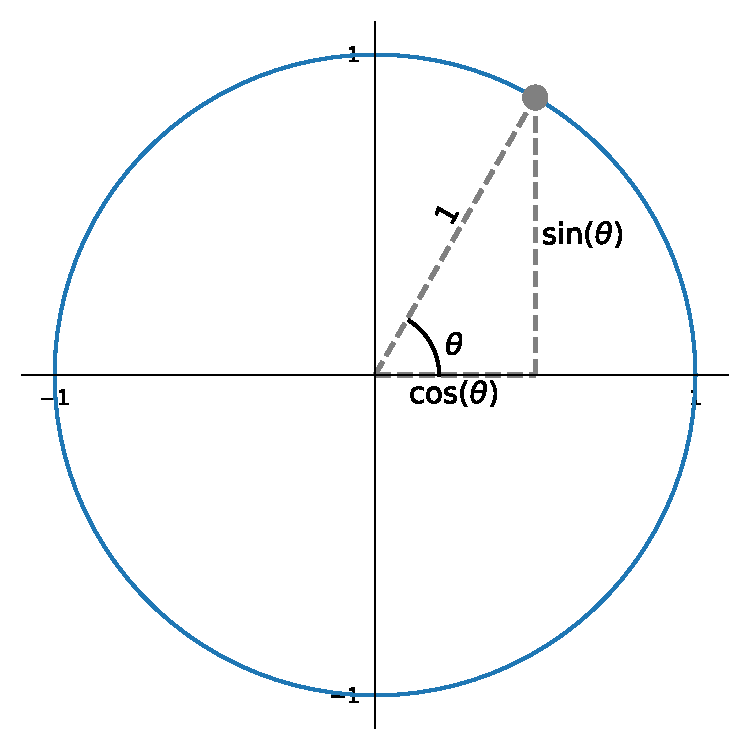
\includegraphics[width = .7\textwidth]{figures/mathplots/unit-circle.pdf}
\end{center}

\pyfile{unit-circle.py}

We can plot a circle or an arc from $\theta_1$ to $\theta_2$, by connecting the points $\left(\cos(\theta_1), \sin(\theta_1)\right), \dots, \left(\cos(\theta_2), \sin(\theta_2)\right)$, where enough intermediate angles between $\theta_1$ and $\theta_2$ are included so the piecewise-linearity is smoothed out to give the appearance of a curve. In Subsection \ref{subsec:nonunit}, we consider how to do the same, but for non-unit circles.


\subsection{Non-unit Circles}\label{subsec:nonunit}

The unit circle has a radius of one and it's centered at the origin. How do we obtain coordinates for other circles? There are two steps to change the radius and shift a circle off the origin. 
\begin{enumerate}
\item \textbf{Change the radius.} Multiply the coordinates by the desired radius $r$.
\item \textbf{Shift the circle.} Add the desired horizontal and vertical shifts to the $x$ and $y$ coordinates, respectively. 
\end{enumerate}
These are ordered because the radius multiplier should not be applied to the added shift term. Below, we shrink the unit circle and move it up and along the 45-degree line.

\pyfile{unit-circle-shift.py}

\begin{center}
    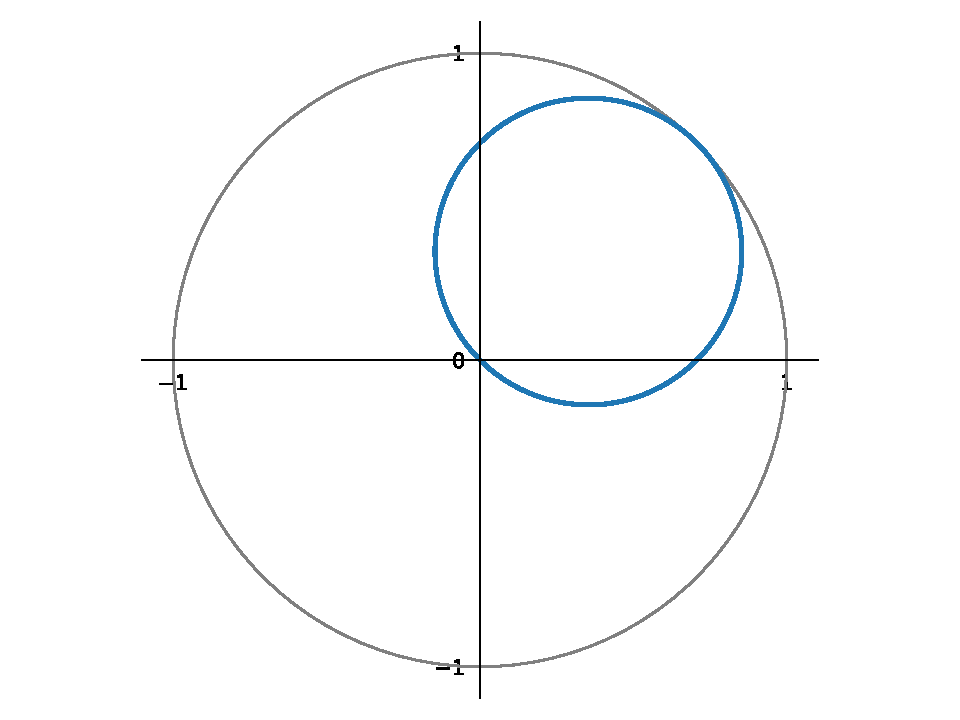
\includegraphics[width = 0.7\textwidth]{figures/mathplots/unit-circle-shift.pdf}
\end{center}

\subsection{Rotations and Ellipses}\label{subsec:rotations}

Now we jump from trigonometry to linear algebra. Matrices can represent transformations, like rotations or stretching. Applied to each point in a circle, a rotation that stretches $x$ and $y$ coordinates differently creates an ellipse.

A rotation of angle $\theta$ can be represented as
$$\left[ \begin{array}{cc}
    \cos \theta & -\sin \theta \\
    \sin \theta & \cos \theta
\end{array} \right].$$ Stretching the $x$-dimension by a scalar $r$ can be represented with
$$ \left[ \begin{array}{cc}
    r & 0 \\
    0 & 1 
\end{array} \right],$$ and the $y$-dimension is stretched by
$$ \left[ \begin{array}{cc}
    1 & 0 \\
    0 & r 
\end{array} \right].$$

Each of these matrices is applied point by point by left multiplying that point (as a $2\times 1$ column vector) by the transformation matrix,
$$ \begin{pmatrix}
     \tilde{x}  \\
     \tilde{y}
\end{pmatrix} = T \begin{pmatrix}
     x  \\
     y
\end{pmatrix}.$$


Below we take a circle and shrink it horizontally, stretch it vertically, and then rotate it. The $x$ values are multiplied by $\frac{1}{2}$, the $y$ values are multiplied by 2, and the angle of rotation is 45 degrees ($\frac{\pi}{4}$ radians). The transformation is constructed below. 

\pyfile{tform-matrix.py}

Below we plot a unit circle and then apply the transformation to create an ellipse.

\pyfile{ellipse-tform}

\begin{center}
    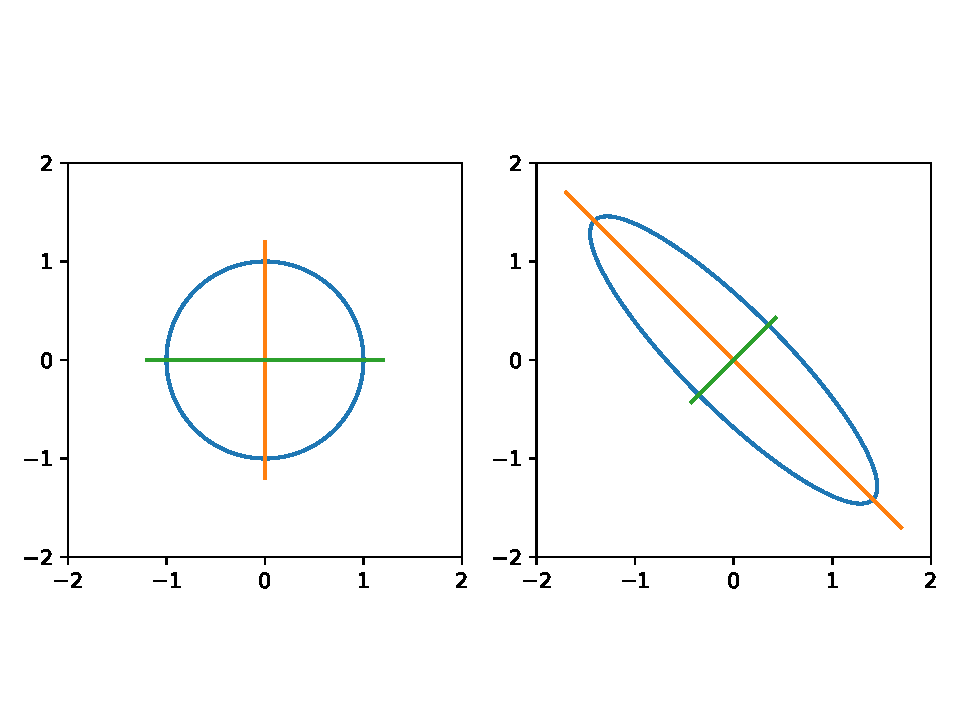
\includegraphics[width = .7\textwidth]{figures/mathplots/ellipse-tform.pdf}
\end{center}



\section{Right Triangles}

Right triangles are important to understand not for plotting right triangles necessarily, but for understanding the angle between any two points. The line segment connecting two points forms the hypotenuse of a right triangle, just as was seen in the unit circle. 

For any angle $\theta$ in a right triangle that is not the right angle itself, we can speak of the sides opposite or adjacent to the angle. The side opposite is the side directly across from the angle. The side opposite the right angle is the hypotenuse (of length $c$ in Pythogoras' Theorem). The SOHCAHTOA mnemonic helps us understand how side lengths are related to the angles. More clearly written as SOH-CAH-TOA, as it stands for Sine Opposite Hypotenuse Cosine Adjacent Hypotenuse Tangent Opposite Adjacent and means 

\begin{align*}
    \sin \theta & = \frac{\text{opposite}}{\text{hypotenuse}} & \\ 
    \cos \theta & =  \frac{\text{adjacent}}{\text{hypotenuse}} &\\ 
    \tan \theta & = \frac{\text{opposite}}{\text{adjacent}}, &
\end{align*}

\noindent where $\theta$ is some angle of a triangle in radians and opposite, adjacent, and hypotenuse refer to the lengths of these sides. 

By understanding these functions and their inverses, we can recover the angles in a plot. These functions are available from the \code{math} module as \code{sin()}, \code{cos()}, and \code{tan()}. Their inverses are \code{asin()}, \code{acos()}, and \code{atan()} for $\arcsin$, $\arccos$, and $\arctan$. 

\code{math.atan()} is the most useful. Take two points and the slope $m$ of the line connecting them. Then $\arctan(m) = \theta$ is angle between those points, in radians. 

\pyfile{r-triangle.py}

\begin{center}
    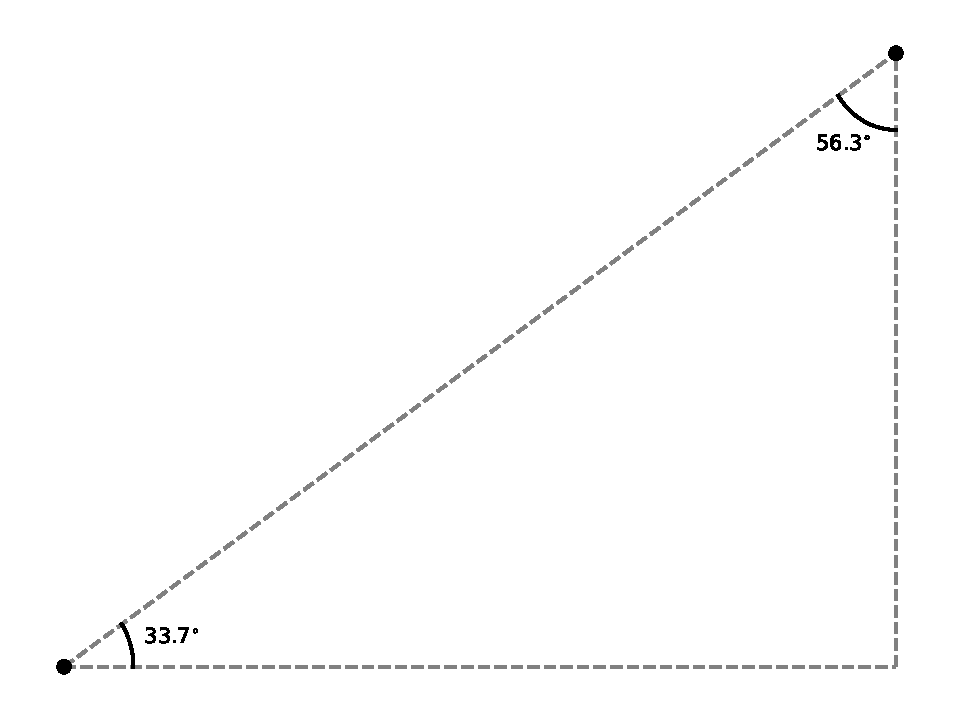
\includegraphics[width = .7\textwidth]{figures/mathplots/r-triangle.pdf}
\end{center}


%\begin{center}
 %   \includegraphics[width = .7\textwidth]{mathplots/slope_and_tangent.pdf}
%\end{center} % find the code for this


\chapter{Applications}\label{chapter:mathapp}

\section{Sloping Text}\label{sec:slopingtext}

Suppose you'd like to label a line. 

For a sloped line, you might rather the text sit parallel to the line instead of suffering the below.

\pyfile{no-slope.py}

\begin{center}
    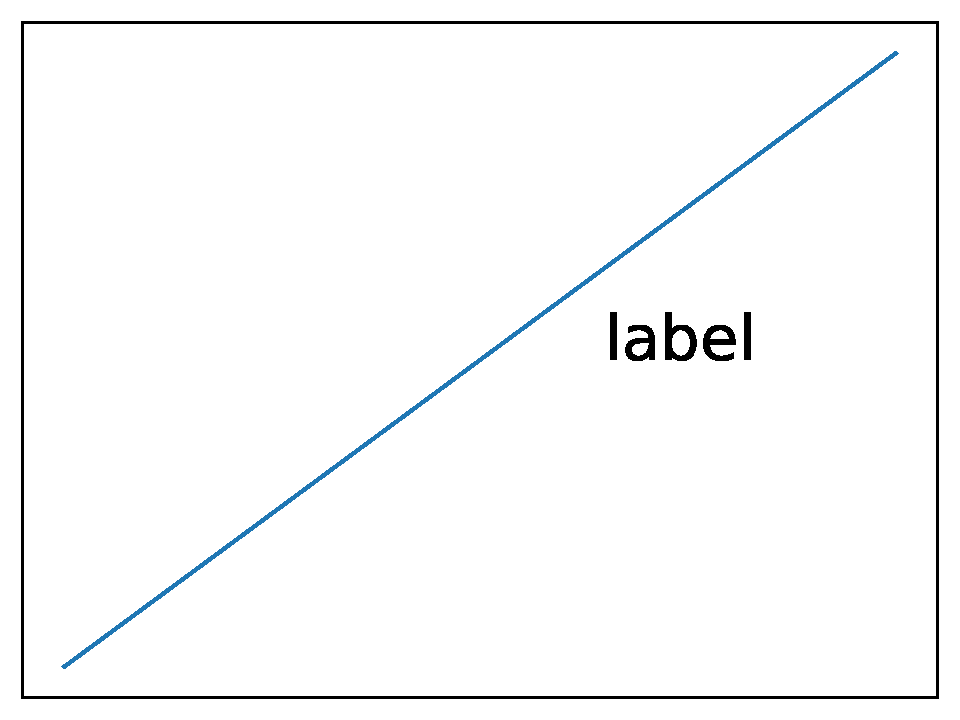
\includegraphics[width = .6\textwidth]{figures/mathplots/no-slope.pdf}
\end{center}

The \code{rotation} argument can help if you know the right angle in degrees. Here the angle is 45 degrees or $\frac{\pi}{4}$ radians. So we modify the second line to be \code{plt.text(0.65, 0.5, 'label', size = 30, rotation = 45)}.

But this doesn't do what we want! The plot coordinate system is stretched, because we didn't call \code{ax.set_aspect('equal')} and \code{text} doesn't recalculate the text angle to make it align. 

\begin{center}
    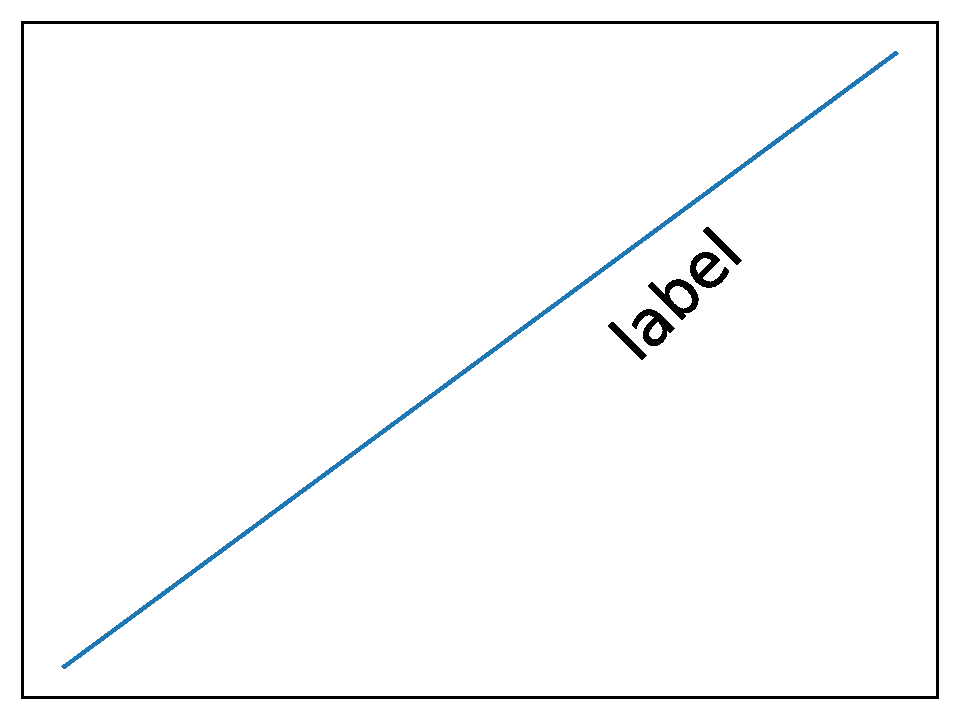
\includegraphics[width = .6\textwidth]{figures/mathplots/bad-slope.pdf}
\end{center}

Now let's solve it for good in the general case, using trigonometry and then \code{transform_angles}. Try experimenting by replacing the \code{x2,y2} values to see this works for any angle.  

\pyfile{slope-label.py}

\begin{center}
    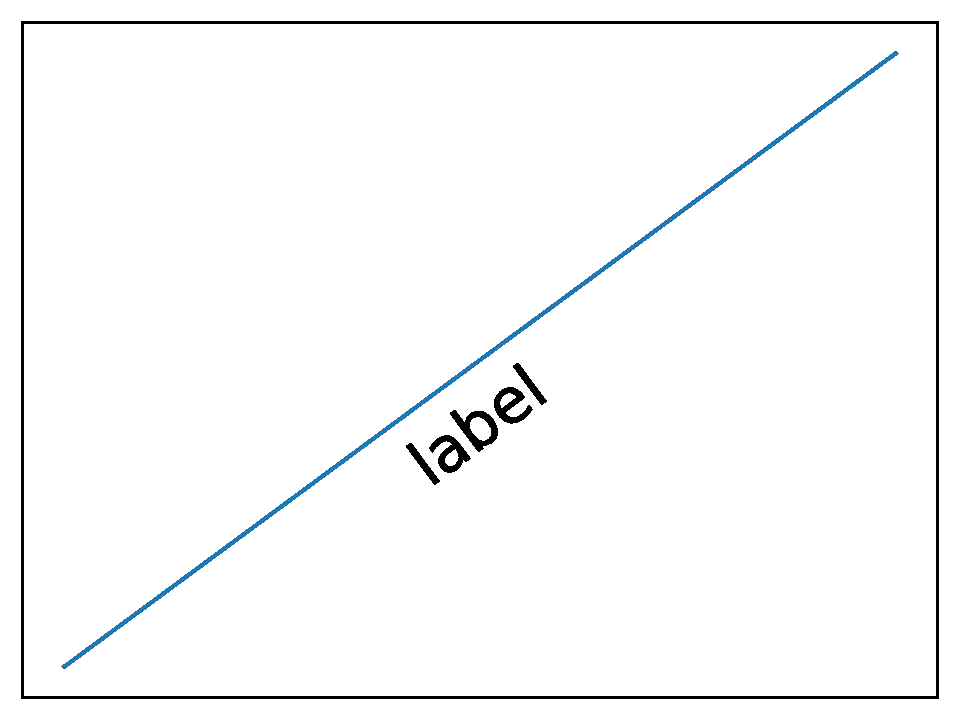
\includegraphics[width = .6\textwidth]{figures/mathplots/slope-label.pdf}
\end{center}

\section{Circular Arrangements}\label{sec:circarrange}

With our knowledge of the unit circle, we can arrange some points in a circle with no additional help beyond the math package. This might be useful if you want to avoid mixing polar and Cartesian axes. 
%https://stackoverflow.com/questions/18789157/matplotlib-combine-polar-and-cartesian-gridded-data
\begin{lstlisting}[language = Python]
n_points = 10
pie_angle = 360/n_points # angle of each slice
starting_angle = 90

fig, ax = plt.subplots()

for i in range(n_points):
    
    angle = starting_angle + i*pie_angle
    angle = math.radians(angle)
    x = math.cos(angle) 
    y = math.sin(angle)
        
    ax.plot([x],[y], 'o', markersize = 17 - i)
    
ax.set_aspect('equal')
ax.axis('off')
\end{lstlisting}

This code produces the following.

\begin{center}
    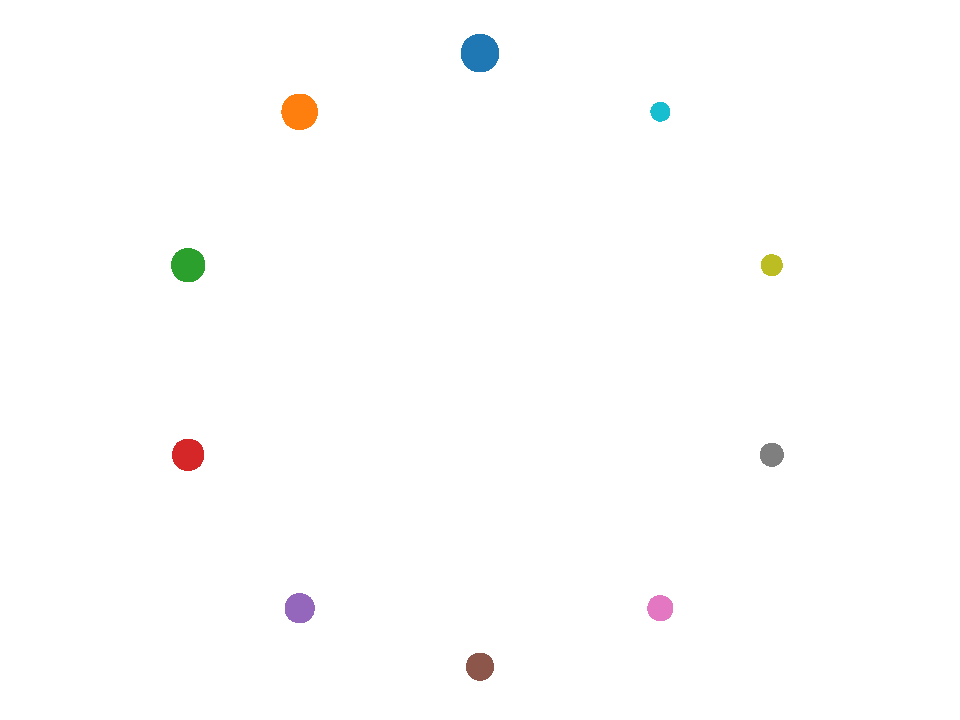
\includegraphics[width = .6\textwidth]{mathplots/circle.pdf}
\end{center}


The below makes similar use of trigonometry to create a circle colored according to a gradient, like in Chapter \ref{chapter:colors}. I make use of \code{solid_capstyle = 'round'} to round the endpoints of the plotted line, creating a cleaner look compared to the default. 

\begin{lstlisting}[language = Python]
# make a circle gradient
start_color = 255/256, 59/256, 48/256 # red
end_color = 255/256, 255/256, 85/256 # yellow

# How many color changes
segments = 130

# Create figure
fig, ax = plt.figure(figsize = (8,8)), plt.axes()

# Start at 90 degrees and return clockwise
angles = np.linspace(2.5*np.pi, np.pi/2, segments + 1)

# Create the intermediate colors
colors = dict()
for i in range(3):
    colors[i] = np.linspace(start_color[i], end_color[i], segments)
    
# plot each arc
for i in range(segments):
    
    start_angle = angles[i]
    end_angle = angles[i+1]
    angle_slice = np.linspace(start_angle, end_angle, 100)
    
    x_values = np.cos(angle_slice)
    y_values = np.sin(angle_slice)
    
    rgb = colors[0][i], colors[1][i], colors[2][i]
    
    ax.plot(x_values, y_values, 
        color = rgb,
        linewidth = 20, 
        solid_capstyle = 'round')

ax.set_aspect('equal')
ax.axis('off')
\end{lstlisting}

\begin{center}
    \includegraphics[width=.8\textwidth]{proseplots/circlegradient.pdf}
\end{center}

\section{Network Graphs}

Networks are represented mathematically as graphs---a set of vertices and edges between them. In drawing a graph, there are many drawing algorithms available. For large networks or sophisticated algorithms, you should use something off the shelf in a package like \link{https://nxviz.readthedocs.io/en/latest/index.html}{nxviz}. For a small network, you might avoid dealing with NetworkX and nxviz and do the drawing yourself. We will work through two simple layouts: arc diagrams and a circular layout for an undirected graph. 

An arc diagram places all points on a straight line. The links are drawn as arcs from one point to another. 

Let's consider the complete graph with four vertices, where every pair is connected. 

\begin{lstlisting}[language = Python]
fig, ax = plt.figure(), plt.axes()
x = np.linspace(0,1,4)
ax.plot(x, np.zeros(4), 
        marker = 'o', 
        linestyle = '',
        markersize = 13)

angles = np.linspace(0,np.pi,100)
for point in x:
    # connect other points
    other_x = x[x > point]
    # construct a half circle
    unit_x, unit_y = np.cos(angles), np.sin(angles)
    for other in other_x:
        shift = np.mean([point,other])
        r = (other - point)/2
        new_x = r*unit_x + shift
        new_y = r*unit_y
        ax.plot(new_x, new_y, zorder = -1)
    
ax.axis('off')
ax.set_aspect(1.5)
\end{lstlisting}

\begin{center}
    \includegraphics[width=.7\textwidth]{mathplots/arcDiagram1.pdf}
\end{center}

Next we move on to a circular layout. This layout places each vertex along a circle. Spaced evenly and with just four vertices in our graph, this will in fact produce a square. We also label each edge. 

\begin{lstlisting}[language = Python]
fig, ax = plt.figure(), plt.axes()

n_points = 4

# Draw vertices
angles = np.linspace(0, 2*np.pi, n_points + 1)[0:n_points]
x = np.cos(angles)
y = np.sin(angles)
ax.plot(x, y, 
        marker = 'o', 
        linestyle = '',
        markersize = 13)

# Draw Edges
points = [p for p in zip(x,y)]
counter = 1
for point, other in combinations(points,2):

    x = [p[0] for p in (point, other)]
    y = [p[1] for p in (point, other)]
    ax.plot(x, y, zorder = -1)

    # add a label
    label_point = .65*np.array(point) + .35*np.array(other)

    run = x[1]-x[0]
    rotation = 90
    ha = 'left'
    if run != 0:
        line_slope = (y[1]-y[0])/(x[1]-x[0])
        rotation = math.atan(line_slope)
        rotation = math.degrees(rotation)
        ha = 'center'
    else:
        print(point, other, rotation)

    # get rgb then blend with white
    line_color = colors.to_rgb("C"+str(counter))
    lighter = .8*np.ones(3) + .2*np.array(line_color)
    ax.text(label_point[0], label_point[1],
            'label', rotation = rotation,
            bbox = dict(facecolor = lighter),
            va = 'center',
            ha = 'center'
           )
    counter += 1
        
ax.axis('off')
ax.set_aspect('equal')
\end{lstlisting}

\begin{center}
\includegraphics[width = .83\textwidth]{mathplots/circleDiagram1.pdf}
\end{center}



\section{Tony Hawk's Vertical Loop}

Tony Hawk became the first skateboarder to skate a vertical loop in 1998. We honor that accomplishment in two dimensions with the help of a rotation matrix. The unit circle is our vertical loop and we add two smaller circles to represent a skateboard. This is trigonometry. The small circles are placed along a ray from the origin of the unit circle to ensure they will lie tangent inside in the loop. In the first subplot, we place the skateboard at the bottom of the ramp. Though the same figure could be produced without using a rotation matrix, we use one so that the first subplot is essentially reused over and over by rotating the skateboard wheels up and around the loop.

%https://ftw.usatoday.com/2018/08/skater-lizzie-armanto-makes-history-by-completing-tony-hawks-loop

\begin{lstlisting}[language = Python]
thetas = np.linspace(0,2*np.pi,8)[0:-1]
fig = plt.figure(figsize = (12,3))

# Set radius for skateboard wheels
radius = 0.1

# Make individual subplots
for key, theta in enumerate(thetas): 
    rotation_matrix = np.matrix([[np.cos(theta), -np.sin(theta)], [np.sin(theta), np.cos(theta)]])

    # Create panel for one frame
    ax = fig.add_subplot(1, len(thetas), key+1)
    ax.set_aspect('equal')

    # Plot the loop itself
    angles = np.linspace(0, 2*np.pi, 100)
    x = np.cos(angles)
    y = np.sin(angles)
    ax.plot(x,y)

    # Make skateboard wheels at bottom of the ramp
    # and then rotate them counter-clockwise according to theta
    centers = list()
    for ang in 1.5*np.pi, 1.6*np.pi:      
        center = (1-radius)*np.cos(ang), (1-radius)*np.sin(ang)

        # rotate 
        point = np.matrix(center).T
        rotated_point = rotation_matrix*point
        rotated_point = np.array(rotated_point).flatten()
        centers.append(rotated_point)
        
        # make wheel around new center
        wheel_x = radius*x + rotated_point[0]
        wheel_y = radius*y + rotated_point[1]

        ax.plot(wheel_x, wheel_y)

    # connect the two wheel centers
    c1, c2 = centers
    ax.plot([c1[0],c2[0]], [c1[1],c2[1]])
    
    ax.axis('off')
    
    xlim = ax.get_xlim()
    ax.plot(xlim, [-1,-1], color = 'C0', zorder = -1)
\end{lstlisting}


\begin{center}
    \includegraphics[width = \textwidth]{mathplots/TonyHawkLoop.pdf}
\end{center}
